\section{Situation \& Problems}
%situation:
\begin{frame}[t]{Current situation}
\begin{columns}[T]
\column{0.6\textwidth}
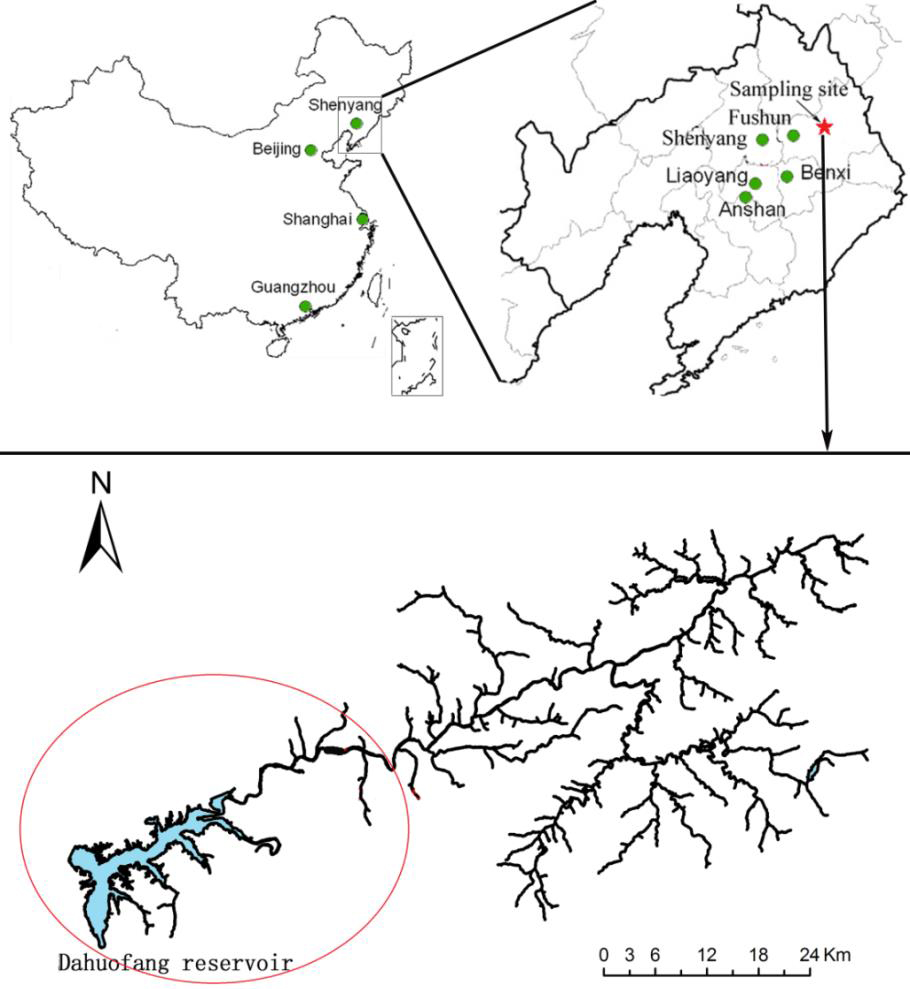
\includegraphics[height=0.95\textheight]{study_area.jpg}
\column{0.4\textwidth}
	\begin{itemize}		
		\item Water source of city group in the lower reaches
		\item 110 $km^2$, 7 bil.\ $m^3$ water for \alert{12 mil.} people per year
	\end{itemize}
\end{columns}
 \end{frame}

%problems:
\begin{frame}[t]{Main problems}
	\begin{itemize}[<+- | alert@+>]
		\item Water pollutants: NH$_3$-N (9.73 mg/L, 3.87 times higher) and TP (0.84 mg/L, 1.1 times higher)
		\item River bank damaged, riparian vegetation destroyed
		\item Wetland degraded, soil and water conservation capacity decreased
		\item Water-conservation-stands (WCS) structure single and simple, ecological functions lost
	\end{itemize}

\begin{columns}[T]
	\column{0.33\textwidth}
	\uncover<2->{\alert<2>{\frame{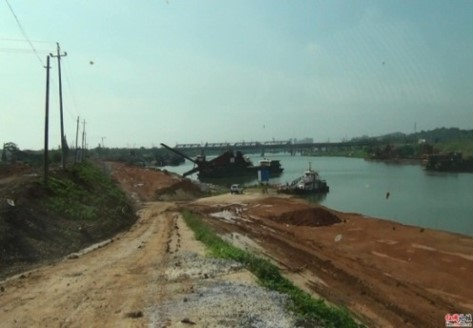
\includegraphics[width=\textwidth]{river_bank_damaged.jpg}}}}
		
	\column{0.33\textwidth}
	\uncover<3->{\alert<3>{\frame{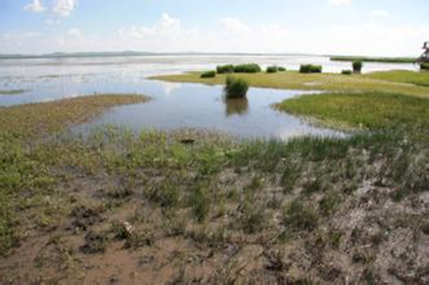
\includegraphics[width=\textwidth]{wetland_degraded.png}}}}	
	
	\column{0.33\textwidth}
	\uncover<4->{\alert<4>{\frame{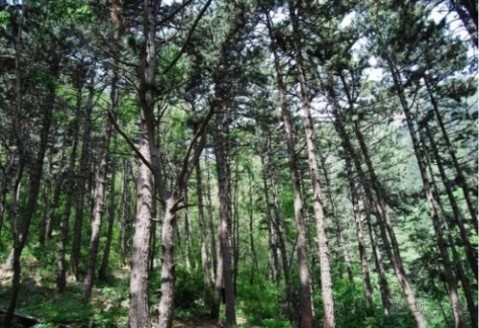
\includegraphics[width=\textwidth]{water_conservation_stands_structure_single.jpg}}}}
\end{columns}
\end{frame}